%
% File naaclhlt2015.tex
\documentclass[11pt,letterpaper]{article}
\usepackage{naaclhlt2015}
\usepackage{enumitem}
\usepackage{times}
\usepackage{latexsym}
\setlength\titlebox{6.5cm}    % Expanding the titlebox
\usepackage{latexsym,graphicx,algorithmic}

\usepackage{todonotes}
\usepackage{url}

\usepackage{tikz-dependency}
\usepackage{pifont}

\usepackage{xcolor,colortbl}%to color cells

%handy shortcuts
\newcommand{\baseline}{{\sc Baseline}}
\newcommand{\tab}[1]{\hspace{.2\textwidth}\rlap{#1}}

\renewcommand{\theequation}{\thesubsection\arabic{equation}}

\usepackage{amsfonts}
\usepackage{graphicx}

%SemEval-2015 System Description Paper
%Paper Title:  The title should follow the pattern "<TEAM_ID> :  <Paper Title>"  where <TEAM_ID> is the team ID used when registering with SemEval-2015 and <Paper Title> is the title of your paper.
%Page Limit:  A system description paper has up to 4 pages of content + 2 pages for references. 
%Papers should describe the methods used clearly, and in sufficient detail in order to ensure reproducibility.

\title{CPH: TITLE}

\author{Sarah McGillion\\
	    University of Copenhagen\\
	    111 Anywhere Street\\
	    Mytown, NY 10000, USA\\
	    {\tt zhg159@xyz.org}
	  \And
	Barbara Plank\\
  	University of Copenhagen\\
  	900 Main Street\\
  	Ourcity, PQ, Canada A1A 1T2\\
  {\tt author2@abc.ca}
	 \And
	Hector\\
  	University of Copenhagen\\
  	900 Main Street\\
  	Ourcity, PQ, Canada A1A 1T2\\
  {\tt author2@abc.ca}}

\date{}

\begin{document}
\maketitle
\begin{abstract}
 
\end{abstract}

\section{Introduction}
This paper outlines the methods used to build a model that could score the sentiment of figurative language used in twitter, not only to a three class situation, positive, negative and neutral, but to be able to find a fine grained integer score in the range [-5,5], where -5 would represent the most negative sentiment for a tweet. The systems described attempted to do this without the use of explicit sentiment lexicon. For two of the systems described the results of a general sentiment analyser (based on the work of Elming {\it et al}. (2014)) were used as features, as early tests showed that this type of general sentiment tool could not be directly used for this task. No exploration of sentiment lexicon was performed and therefore no explicit semantic lexical features were used in the models outlined, instead lexicons were used implicitly through the general sentiment analyser, as predictions from this tool were used as features for the systems and in one case, used as a back off score when a tweet could not be identified as coming from a known figurative language type, as identified through analysis of the training data. In the second of such systems the system would back off to a score from the general sentiment analyser to change the predictions for tweets that were recognised as potentially not coming from a known distribution of figurative tweets. This task was addressed as a regression task, but some experiments were conducted with classification algorithms to assess different strengths of the methods. 


\section{System Description}

\subsection{Constant baselines}
Four baseline systems were constructed. These were the Mean, Mode, Median and Random baseline systems. The results of these systems can be seen below in Table \ref{tbl:baselines}. It is interesting to note that while cosine similarity scores can be the same, the mean squared error (MSE) can differ and as such when assessing the performance of systems developed for this task it was not only the cosine similarity measure that was used, but also the MSE.

\begin{table}[ht!]
%\resizebox{\columnwidth}{!}{
\begin{center}
\begin{tabular}{|l|r|r|}
\hline
System & Cosine & MSE\\
\hline
Mean & 0.73 & 3.13\\
Mode & 0.73 & 3.13\\
Median & 0.73 & 3.31\\
Random & 0.59  & 5.17\\
\hline
\end{tabular}
\end{center}
%} % end resize box
\caption{Baseline Results on Trial Data.}
\label{tbl:baselines}
\end{table}

\subsection{Tweet Label System}
A regular expression decision list classifier was implemented to assign a 'type' to a tweet as belonging to a certain class of tweet. The expressions used to find the label for a tweet can be seen below in Table \ref{tbl:tweettype}. The system searched for the expression in a tweet and then would assign a label to the first expression that was found, the order of the decision list follows that in Table \ref{tbl:tweettype} starting from the top left column to the bottom right column, where if no type could be found then the tweet was assigned a 'NoLabel' label.

\begin{table}[ht!]
\resizebox{\columnwidth}{!}{
\begin{tabular}{|l|l||l|l|}
\hline
Label & Expression & Label & Expression  \\
\hline
Sarcasm & \#sarcas & SoToSpeak & so to speak\\
Irony & \#iron(y \ ic)  & Proverbial & proverbial\\
Not & \#not & JustKidding & \#justkidding \\
Literally & literally & Not2 & not \\
Virtually & virtually & about & about \\
YeahRight & \#yeahright &  Oh & oh \\
OhYouMust & Oh.*you & NoLabel & - \\
asXas & as .* as & &\\
\hline
\end{tabular}
} % end resize box
\caption{Tweet Label Type and Expression.}
\label{tbl:tweettype}
\end{table}

\subsection{Regression models}
<<<<<<< HEAD
As stated above the true sentiment scores we chose to work with were floating point scores that gave the average human annotated scores for the tweets. Approaching the labelled data in this way led to a regression system setup.
The regression systems are as follows; N-Gram Linear Regression, Multi feature  Ridge Regression, PCA\_GMM Ridge Regression and Embeddings with Bayesian Ridge. The features and models used for these systems shall be described briefly below. The preprocessing methods were the same across the models, excluding Tweet Label Regression. Experiments were run to determine if stopwords or the removal of stopwords affected performance, similarly with usernames. These experiments showed that the removal of stopwords increased the performance, and a decision was made to replace usernames with a single shared word 'USER' .  The following gives a short description of the systems and results for these regression models can be found in Table \ref{tbl:regressionResults}

\subsubsection{N-gram Linear Regression (LR)}
\label{subsec:LR}
A linear regression system was experimented with, it used as features count, binary presence or tf-idf normalized counts of  n grams of varying size. The best of such systems used the counts of 1,2 and 3 word grams. 

\subsubsection{Multi Feature Ridge Regression (RR)}
\label{subsec:RR}
The features used for this model were 1 and 5 word grams, counts of the number of words that were all uppercase, some punctuation features: number of contiguous sequences of exclamation marks, question marks and exclamation marks and questions marks and the tweet label assigned from the Tweet Label System.

\subsubsection{PCA\_GMM Ridge Regression (GMM)}
\label{subsec:GMM}
The features used were a binary bag-of-words features from 1, 2, and 3  word grams. PCA was used to reduce the dimensionality to 100, and Gaussian Mixture Models (GMM) were used to find underlying distributions in the data, here 12 Gaussians were assumed.{ \bf  The GMM was used under the assumption that the data in the set came from many types of figurative language, and were therefore sampled from different distributions}

\subsubsection{Embeddings with Baysian Ridge (EMBD)}
\label{subsec:EMBD}
The embeddings were built on: a tweet corpus sampled with the labels from theTweet Label System, the training data, some key words that were identified from a data exploration of the test data for example `speak'. The corpus was lowercased and the usernames and URLs in the corpus were normalized to '@USER' and 'URL' respectively. This resulted in a total of 3.7 million tweets and 67 million tokens.\newline
The gensim library was used to create the word embeddings and the parameters for creating these embeddings were: 100 dimensions, 5 minimum occurrences for a type to be included in the mode, 5 word context window and 10-example negative sampling.\newline
Each tweet was represented by 100 features that represented the average of all the embeddings of the content words in the tweet. The learner used was a Bayesian Ridge Regressor with standard parameters as found in sklearn.

\subsubsection{Regression Model Results}
Table \ref{tbl:regressionResults} shows the performance of these systems on the trial evaluation data provided.

\begin{table}[ht!]
%\resizebox{\columnwidth}{!}{
\begin{center}
\begin{tabular}{|l|r|r|}
\hline
System & Cosine & MSE\\
\hline
RR & 0.88 & 1.60\\
LR & 0.87 &1.67\\
GMM & 0.79  & 2.55\\
EMBD & 0.78 & 2.64\\
\hline
\end{tabular}
%} % end resize box
\end{center}
\caption{Regression Model Results on Trial Data.}
\label{tbl:regressionResults}
\end{table}

Figures \ref{fig:LabelPlot.Sarc,soto,asX}, \ref{fig:LabelPlot.lit,prov,yeahright} , and \ref{ig:dontyou,iron,not,not2} show the predicted scores versus the gold values for tweets from the ridge regression system (RR). Then labels were assigned to the tweet ids for these prediction results and the predictions were plotted against the gold scores for the trial data. This allowed an inspection of the performance of the models on particular labels, but also an inspection on the gold label behaviour of the different types of tweets identified. It can be seen in Figure \ref{fig:LabelPlot.Sarc,soto,asX} that the `Sarcastic' tweets have a generally negative sentiment cloud and that the system predicts reasonably well for this type of tweet. Other labels, for example `SoToSpeak' have more variation and spread of the scores for this type of figurative tweet.


\begin{figure}[ht!]
    \centering
    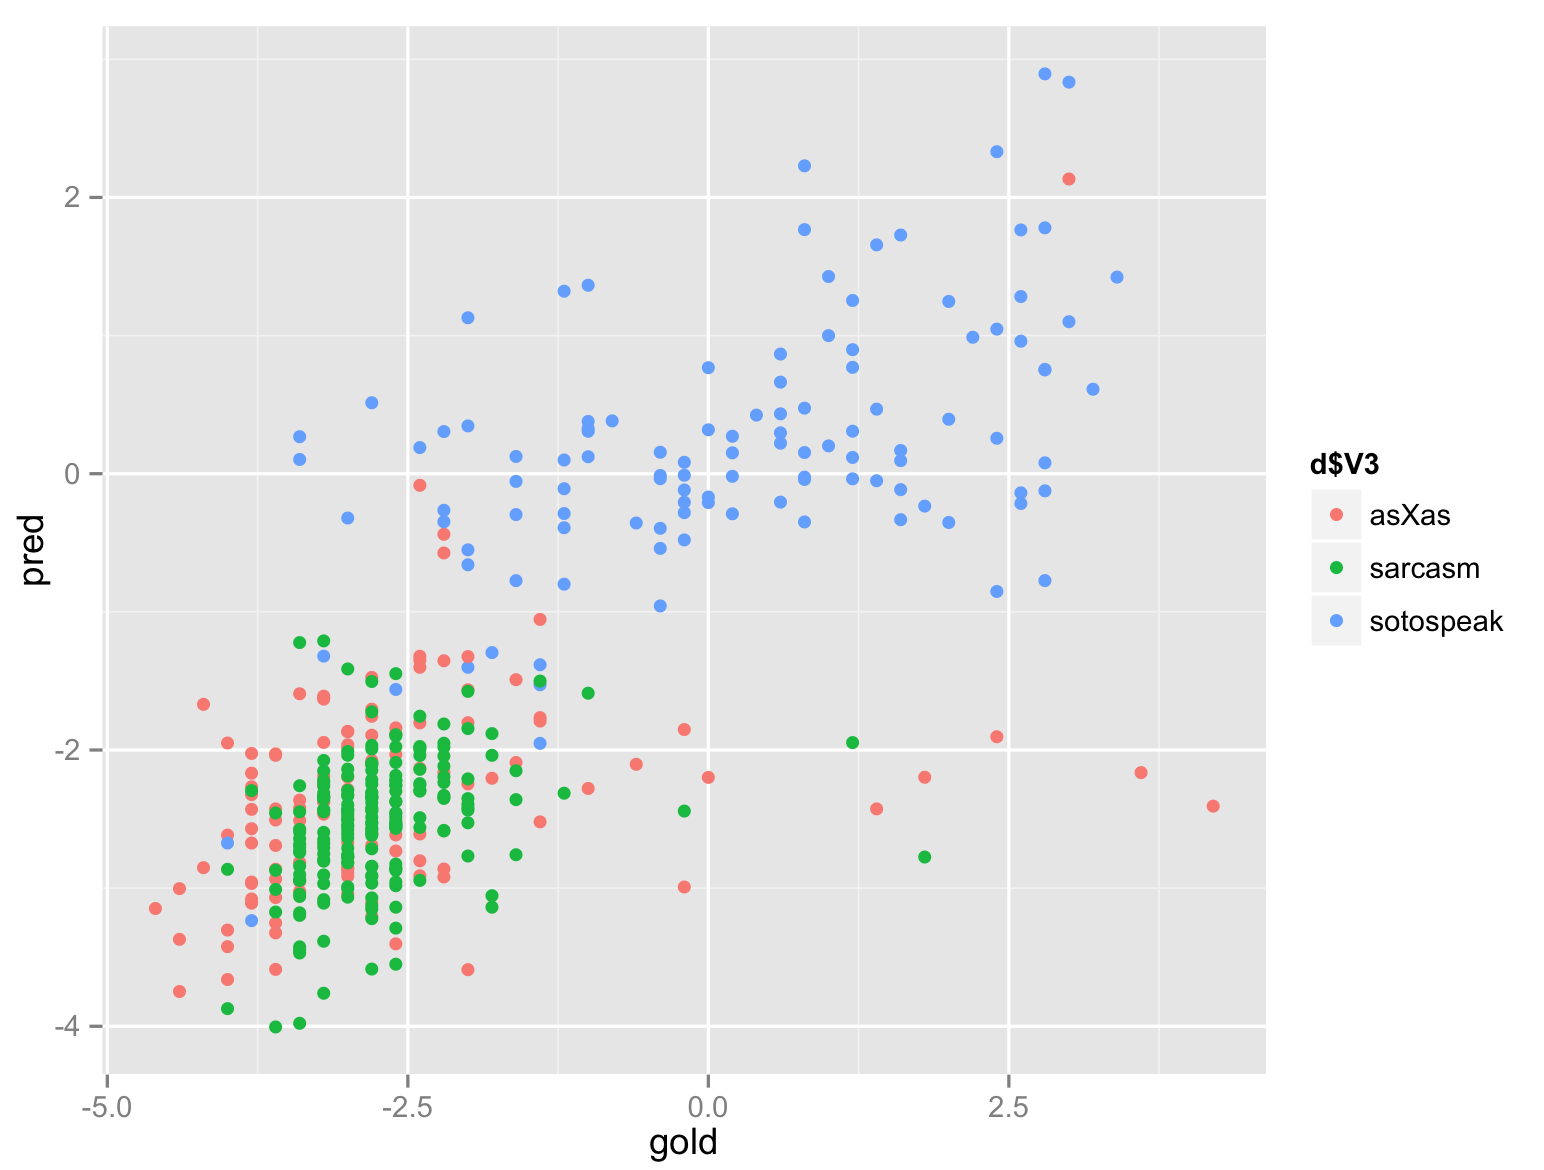
\includegraphics[width=\columnwidth]{labelPlot_sarc_sotoSpeak_asXas.png}
    \caption{Label Plots for RR predictions:}
    \subcaption{ \small Sarcasm, SoToSpeak, asXas.}
    \label{fig:LabelPlot.Sarc,soto,asX}
\end{figure}

\begin{figure}[ht!]
    \centering
    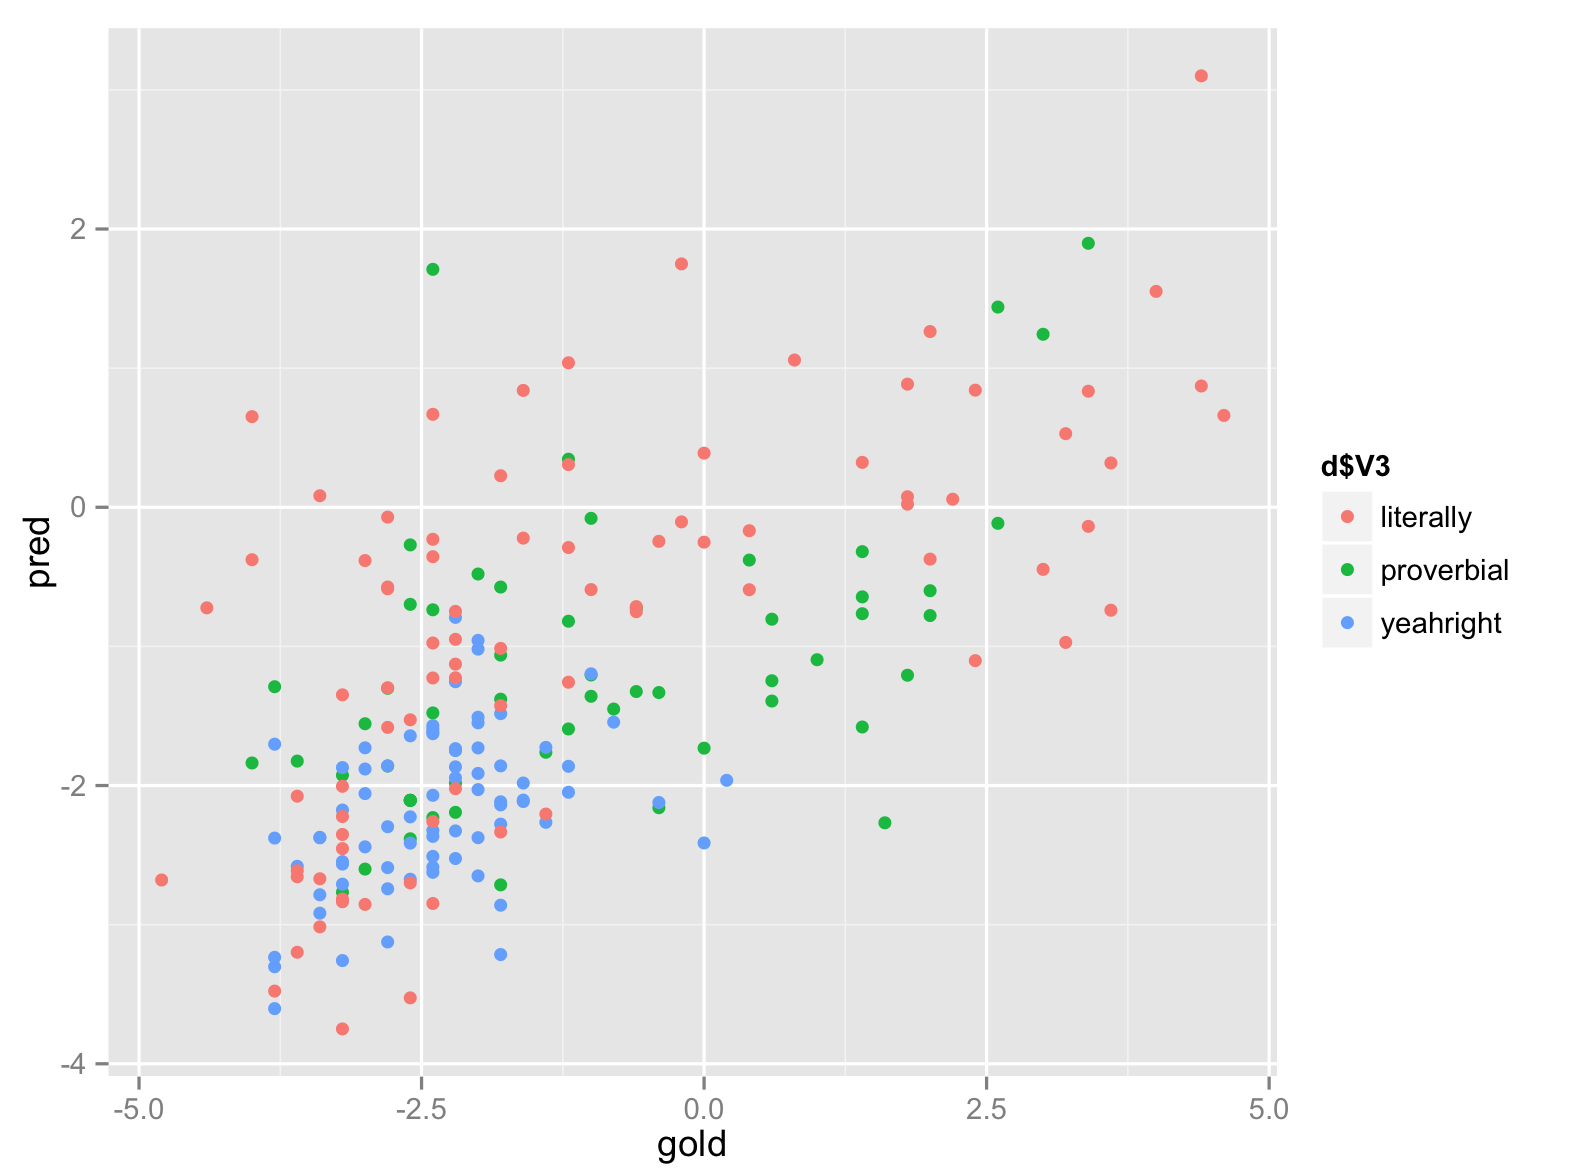
\includegraphics[width=\columnwidth]{labelPlot_literally_proverb_yeahright.png}
    \caption{Label Plots for RR predictions:}
    \subcaption{ \small  Literally,Proverbially,YeahRight}
    \label{fig:LabelPlot.lit,prov,yeahright}
\end{figure}

\begin{figure}[ht!]
    \centering
    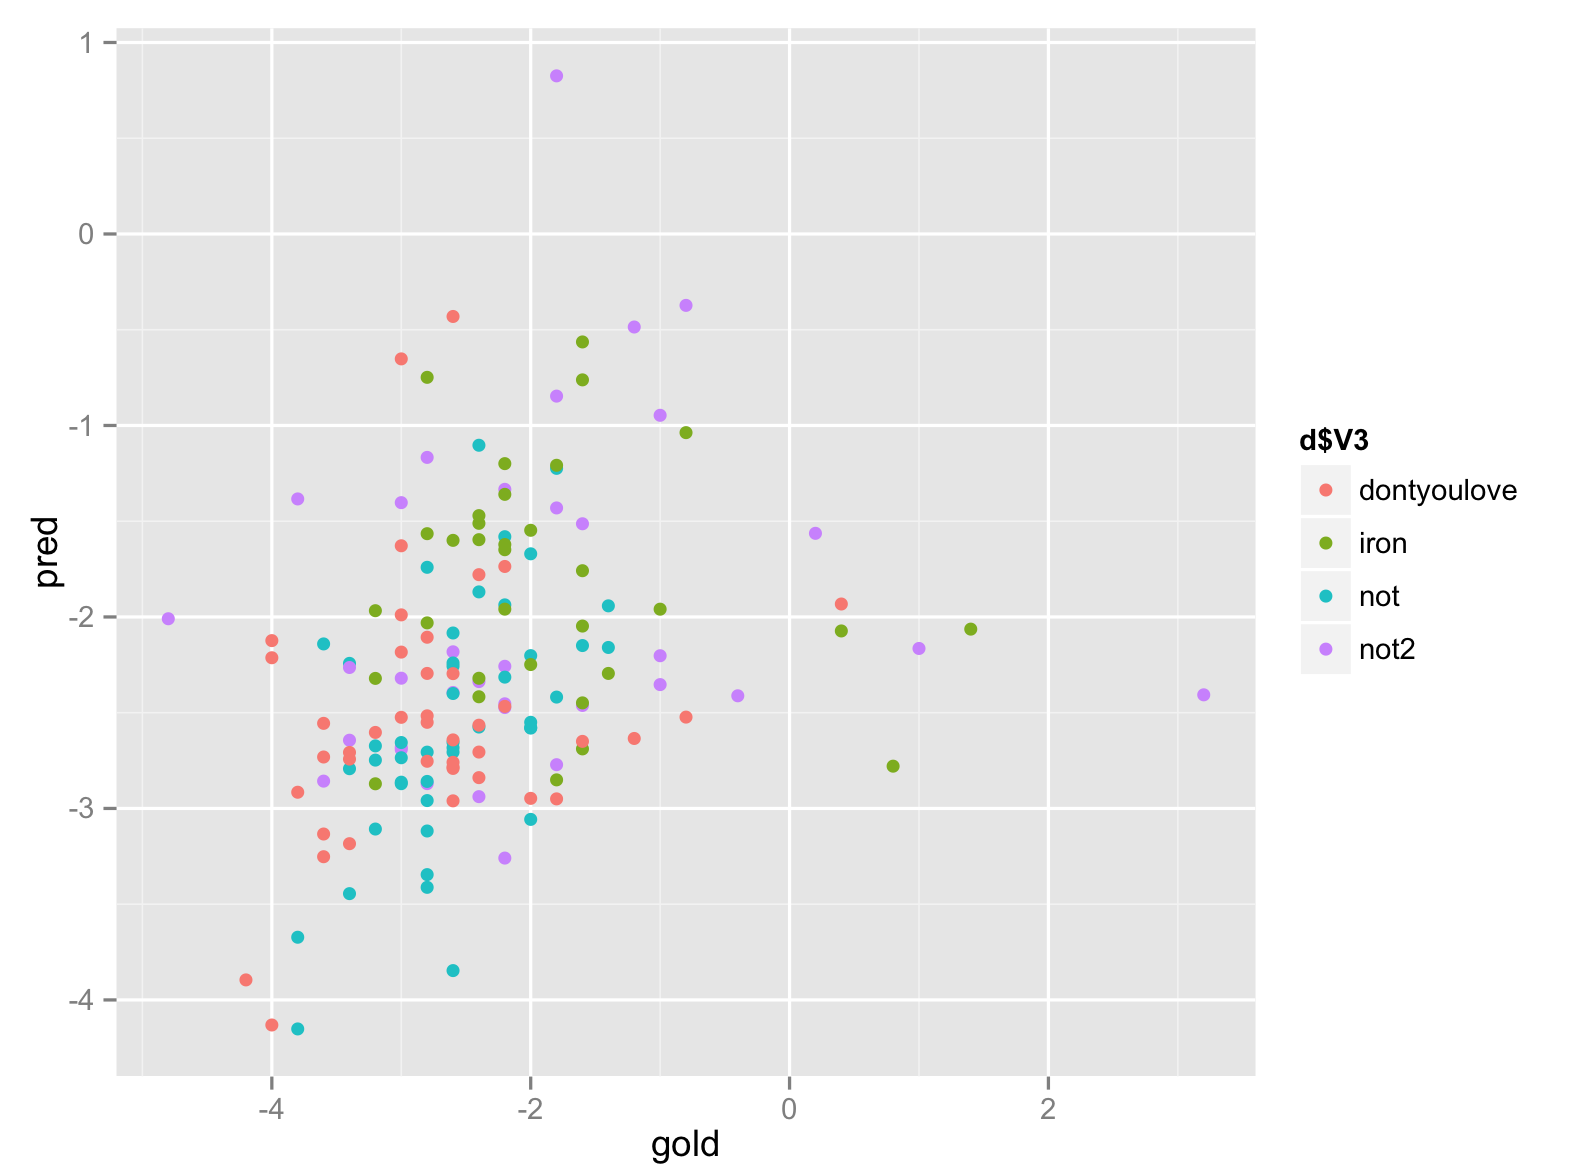
\includegraphics[width=\columnwidth]{labelPlot_dontyou_iron_not_not2.png}
    \caption{Label Plot  for RR predictions:}
    \subcaption{ \small DontYouLove,Irony,Not,Not2.}
    \label{fig:dontyou,iron,not,not2}
\end{figure}
=======
As stated above the true sentiment scores we chose to work with were floating point scores that gave the average human annotated scores for the tweets. Approaching the labeled data in this way led to a regression system setup.
The regression systems are N-Gram Linear Regression, Multi feature  Ridge Regression, Tweet Label Regression, PCA\_GMM Ridge Regression and Embeddings with Baysian Ridge. The features and models used for these systems shall be described briefly below. The preprocessing methods are the same across the models, excluding Tweet Label Regression. Experiments were run to determine if stopwords or the removal of stopwords affected performance, similarly with usernames. These experiments showed that the removal of stopwords increased the performance, and a decision was made to replace usernames with a single shared word 'USER' .  The following gives a hosrt description of the systems and results for these regression models can be found in Table \ref{tbl:regressionResults}

\subsubsection{N-gram Linear Regression (LR)}
A linear regression system was experimented with, it used as features count, binary presence or tf-idf normalized counts of  n grams of varying size. The best of such systems used the counts of 1,2 and 3 word grams. 

\subsubsection{Multi Feature Ridge Regression (RR)}
The features used for this model were 1 and 5 word grams, counts of the number of words that are all uppercase, some punctuation features: number of contiguous sequences of exclamation marks, question marks and exclamation marks and questions marks and the tweet label assigned from the Tweet Label System.

\subsubsection{Tweet Label Regression (TWLR)}
Tweets were assignment a label from the Tweet Label System and then the predicted numerical value for test data was the average in that category in the training data, for example the average score across the 2139 `sarcastic' tweets was -2.34. Although this was a simple system it resulted in a cosine similarity score of 0.81 for the evaluation data.

\subsubsection{PCA\_GMM Ridge Regression (GMM)}

\subsubsection{Embeddings with Baysian Ridge (EMBD)}

\subsubsection{Regression Model Results}
\begin{table}[ht!]
%\resizebox{\columnwidth}{!}{
\begin{tabular}{|l|r|r|}
\hline
System & Cosine & MSE\\
\hline
RR & 0.88 & 1.60\\
LR & 0.87 &1.67\\
TWLR & 0.81 & 2.34\\
GMM & 0.79  & 2.55\\
EMB & 0.78 & 2.64\\
\hline
\end{tabular}
%} % end resize box
\caption{Regression Model Results.}
\label{tbl:regressionResults}
\end{table}

>>>>>>> 932671fb22e1d4f51f338a345a9b2396691d8df5
 
\subsection{Classification models}
\label{subsec:classification}
Although seen primarily as a regression task, experiments were conducted with different types of classification models to compare predictions for this type of setup to the predictions found using regression models.

\subsubsection{General Sentiment Analyser (GSA)}
\label{subsec:GSA}
A General Sentiment Analyser based on the work of Elming et al (2014) was used. The features for this model are outlined in Table \ref{tbl:elmingFeats}. This model classified to be a three class problem, finding sentiment to be positive (+1) , negative (-1) or neutral (0). It also provided scores for how positive, negative and neutral a tweet was. Computing a weighted average of these scores the predictions of this classifier were assigned a value in the range [-5.0,5.0] . The General Sentiment Analyser was trained on 1466 negative 4602 neutral 3660 positive from a different Tweet Corpus. The GSA predicted 553 positive and 367 negative tweets on trial data. The predictions for the scores for this type of figurative language task showed that this model was not suitable. The GSA has a cosine similarity score of -0.08 and MSE of 18.62. for the predictions and the gold vales for the trial data. 


\begin{table}[ht!]
\resizebox{\columnwidth}{!}{
\begin{tabular}{|l|}
\hline

- N-gram presence for token lengths 1 to 4\\
- Skip-grams (n-gram with one middle word replaced by *) presence for token lengths 3 to 4\\
- Character n-gram presence for entire document string for token lengths 1 to 5\\
- Brown clusters (Brown et al., 1992; Liang, 2005) estimated on the source training data\\
- Number of words with only upper case characters\\
- Number of contiguous sequences of question marks, exclamation marks, or both\\
- Presence of question mark or exclamation mark in last word\\
- Number of words with characters repeated more than two times e.g. ’sooooo’\\
- Number of negated contexts using algorithm described in the text\\
- Most positive, most negative, or same amount of polar words according to a sentiment lexicon\\

\hline
\end{tabular}
} % end resize box
\caption{Features used in General Sentiment Analyser. Taken from Elming et al (2014).}
\label{tbl:relmingfeats}
\end{table}
 
\subsubsection{Tweet Label Classifier (TWLC)}
Tweets were assignment a label from the Tweet Label System and then the predicted numerical value for test data was the average in that category in the training data, for example the average score across the 2139 `sarcastic' tweets was -2.34. Although this was a simple system it resulted in a cosine similarity score of 0.81 for the predictions on the trail data.

\subsubsection{Other Classification Models}
Three other classification models were used, Decision Trees (DT), Naieve Bayes (NB) and Naieve Bayes Multinomial (NBM). The problem of addressing the number of classes to represent the problem as was addressed by using percentiles, where if the task was modelled as a 3 class problem, all tweets in the training data scored between the 0th and 33rd percentile were assigned to class A, between the 33rd and 66th to class B, etc. Experiments were run to find the best method to bring these class labels back to numeric values between -5 and 5, such as assigning a class the minimum score of all the training tweets in that class. Table \ref{tbl:classificicationResults} outlines the results of these experiments and shows only the best performing system, the number of classes modelled and the method to change the class to a score. Interestingly the best systems all used different methods to change class labels to scores, but also interestingly the number of classes was always below 11, which would be the number of classes in the interval for this overall task.

\subsubsection{Results for Classification Models}
\begin{table}[ht!]
%\resizebox{\columnwidth}{!}{
\begin{tabular}{|l|r|r|r|l|}
\hline
System & Cosine & MSE & no. classes & method\\
\hline
DT & 0.82 & 2.51 & 7 & Min\\
TWLC & 0.81 & 2.34 & 16 & Mean \\
NBM& 0.79 & 2.49 & 6 & Mean\\
NB & 0.78 & 2.74 & 8 & Median\\
GSA & -0.08 & 18.62 & 3 & Weight\\
\hline
\end{tabular}
%} % end resize box
\caption{Classification Model Results on Trial Data.}
\label{tbl:classificicationResults}
\end{table}



\subsection{Stacking}
Stacking was used to combine the predicted scores from different systems to predict an overall score. Stacking uses a `Meta Learner' to weight the predictions from different systems and learns which systems to `trust' more to provide an overall final prediction score. The predications on the test data by the different systems were used as the features for the test set in the Meta Learner. The training data predictions were found by using cross validation, here 10-fold cross validation was used to get the predictions of the different systems on the training data. Two different stacking systems were implemented and they are described below in Sections \ref{subsubsec:stacking1} and \ref{subsubsec:stacking2}.

\subsubsection{Stacking System 1}
\label{subsubsec:stacking1}
The systems used here were: 
\begin{itemize}
 \item Ridge Regression (RR) as described in Section \ref{subsec:RR} 
 \item Predictions from the General Sentiment Analyser (GSA). Described in Section \ref{subsec:GSA}
\item PCA\_GMM Ridge Regression (GMM) . Described in Section \ref{subsec:GMM}
 \end{itemize}

The Meta Learner used was Linear Regression.

\subsubsection{Stacking System 2: Stacking with Back Off}
\label{subsubsec:stacking2}
A second stacking system was implemented using the following systems outputs as features:
\begin{itemize}
 \item Ridge Regression (RR) as described in Section \ref{subsec:RR} 
 \item Predictions from the General Sentiment Analyser (GSA). Described in Section \ref{subsec:GSA}
\item Embeddings (EMBD). Described in Section \ref{subsec:EMBD}
 \end{itemize}
This system differs from Stacking System 1, not only in the different systems predictions it uses, but because it has an extra `back-off' element. The Tweet Label System was used to categorise the different tweets in the test data and to find any tweets given a `NoLabel' label. Any tweets given this `NoLabel' were assumed to come from a different distribution of tweets and not belonging to a know figurative type. Under this assumption it was regarded that the scores assigned from the General Sentiment Analyser (GSA) may provide a good prediction for these `Other' type of tweets and thus if a tweet was found to have no label, the system would back off the predicted score from the GSA.
This system was implemented with the thought that it could be applied to all kinds of tweets and not only those belonging to a distribution of figurative types. 

\subsubsection{Stacking Results}
The performance of the stacking systems on the trial data can be seen below in Table \ref{tbl:stackingResults}. Stacking System 2 did not perform very well on the trial data but a reason for this is that only 6\% of the trial data was found as not belonging to a known figurative type of tweet.

\begin{table}[ht!]
\begin{center}
%\resizebox{\columnwidth}{!}{
\begin{tabular}{|l|r|r|}
\hline
System & Cosine & MSE\\
\hline
Stacking 1 & 0.856 &1.880\\
Stacking 2 & 0.786 & 2.567\\
\hline
\end{tabular}
\end{center}
%} % end resize box
\caption{Stacking Model Results on Trial Data.}
\label{tbl:stackingResults}
\end{table}



\section{Data}
\label{sec:data}
The training data contained 8000 figurative tweets, which were broken down into 5000 sarcastic, 1000 ironical and 2000 metaphorical tweets. The trial data provided contained trial data contained 1000 tweets. The final test data contained 4000 tweets. Table \ref{tbl:amountdata} shows the number of available tweets and those which were successfully downloaded and used when building the systems.

\begin{table}[ht!]
%\resizebox{\columnwidth}{!}{
\begin{center}
\begin{tabular}{|l|r|r|}
\hline
Dataset & Provided & Downloaded\\
\hline
Train & 8000  & 7988\\
Trial  & 1000  & 920   \\
Test  & 4000  & 4000  \\
\hline
\end{tabular}
%} % end resize box
\end{center}
\caption{Data.}
\label{tbl:amountData}
\end{table}

The true sentiment values used for training and testing during the development stage of this were the floating point scores released and not the integer value scores until the final submissions were created, then the values were cast to integers using rounding, and any values that fell without the range [-5,5] were brought back into range by assigning any negative value less than -5 to be a score of -5 and similarly with values over 5.


\begin{table}[ht!]
%\resizebox{\columnwidth}{!}{
\begin{tabular}{lrrrrrrr}
                          &     & & \\
xxx\\
\end{tabular}
%} % end resize box
\caption{Statistics on the data.}
\label{tbl:data}
\end{table}

\subsection{Observations}
Using the Tweet Label System it was found that 94\% of the trial data could be labelled with the known label types found in the training set, leaving only 6\% with the `NoLabel'. The Tweet Label System estimated that 25\% of the test data came from an unknown type of distribution with regards to the training data, this was a further motivation for using the Stacking with Back Off System. 


\section{Results}
\label{sec:results}

Three models were submitted for final evaluation on the test data to SemEval Task 11 organisers. The three models used were RR (A), Stacking System 1(B), and Stacking System 2 with Back Off (C).

\begin{table}[ht!]
\resizebox{\columnwidth}{!}{
\begin{tabular}{|l||r|r||r|r|}
\hline
System & Trial Cosine & Trial MSE & Test Cosine & Test MSE\\
\hline
A & {\bf 0.875} &{\bf 1.598} & 0.625 & 3.079\\
B & 0.856 & 1.880 & 0.623 &{\bf  3.078}\\
C & 0.786 & 2.567 & {\bf  0.661} & 3.404 \\
\hline
\end{tabular}
} % end resize box
\caption{Submission System Overall Results.}
\label{tbl:submissionsOverall}
\end{table}

\begin{table}[ht!]
\resizebox{\columnwidth}{!}{
\begin{tabular}{|l||r|r|r|r|r|}
\hline
System & Overall & Sarcasm & Irony & Metaphor & Other\\
\hline
A & 0.625&0.897&0.886&0.325&0.218\\
B & 0.623&{\bf 0.900}& \bf{0.903}&0.308&0.226\\
C & {\bf 0.661} & 0.875 & 0.872 & {\bf 0.453} & {\bf 0.584} \\
\hline
\end{tabular}
} % end resize box
\caption{Submission System Cosine Results for types of Language.}
\label{tbl:submissionsCosineBreakdown}
\end{table}

%\begin{table}[ht!]
%\resizebox{\columnwidth}{!}{
%\begin{tabular}{lrrrrrrr}
%                & Trial & Test  \\
%                \hline
%\baseline & \\
%\end{tabular}
%} % end resize box
%\caption{Statistics on the data.}
%\label{tbl:data}
%\end{table}


\section{Related Work}
\label{sec:relatedWork}

~\newcite{reyes2013multidimensional} proposed...

\section{Conclusions}



%\section*{Acknowledgments}

\bibliographystyle{naaclhlt2015}
\bibliography{biblio.bib}
\end{document}
